% !TEX root = ../../main_without_quantization.tex
\chapter{Neural Networks Compression}
\label{chap:compression}
\section{Introduction}
Model compression encompasses a family of techniques aimed at reducing the computational and memory demands of neural networks while preserving, as much as possible, their predictive performance. These methods are typically applied at the level of layers, submodules, or parameter groups and introduce explicit trade-offs between efficiency metrics and model accuracy. Key objectives include reducing model size, lowering inference latency, decreasing memory bandwidth usage, and accelerating both training and deployment, particularly in resource-constrained environments.

A notable characteristic of modern deep learning models is their heavy overparameterization. In such regimes, compression does not merely remove redundancy but can also act as an implicit form of regularization, mitigating overfitting and occasionally improving generalization performance. This phenomenon has been observed across a variety of architectures, especially in large-scale transformer-based models.

Among the most widely adopted compression strategies are \emph{pruning}, \emph{quantization}, \emph{low-rank factorization}, and \emph{knowledge distillation}. These techniques are not mutually exclusive and are frequently combined in practice. Hybrid compression pipelines leverage their complementary strengths to achieve higher compression ratios and better efficiency–accuracy trade-offs than any single method alone.

\section{Quantization}
\label{sec:quant_fundamentals}

Quantization can be defined as the function of mapping continuous values from a high-precision space to a finite low-precision representation. When it come to  neural networks, this means the act of reducing the bit-width of weights, activations, or, in training settings, gradients~\cite{gholami2022survey}. Since training requires better stability than inference, it is common to use high-precision floating-point representations like FP32 or mixed-precision formats~\cite{krishnamoorthi2018quantizing}. During inference, however, lower bits can still express the required precision to keep accuracy high enough. For this reason, it is effective to use quantization as a way to decrease model size and memory movement~\cite{han2016eie}.

\subsection{Mathematical Formulation}

The aforementioned high-precision to low-precision reduction can be described using a quantization operator. Given an input $x \in \mathbb{R}$, quantization maps $x$ to a finite set of values defined by the bit-width $k$, yielding $2^k$ possible integer levels.

In affine quantization, the real-valued range of interest is first restricted to a clipping interval $[\alpha, \beta]$, so that values outside this interval are clipped to one of the bounds, while values inside are represented using an integer code $x_q$. For an unsigned $k$-bit integer domain, the representable integer range is
\[
  q_{\min} = 0, \qquad q_{\max} = 2^k - 1.
\]
The spacing between two adjacent quantization levels is controlled by the scale $s$, defined as
\begin{equation}
  s = \frac{\beta - \alpha}{q_{\max} - q_{\min}} = \frac{\beta - \alpha}{2^k - 1}.
  \label{eq:quant_scale}
\end{equation}
Since the real interval does not have to begin at zero, an integer zero-point $z$ is chosen such that real zero corresponds to an integer code. In the unsigned case,
\begin{equation}
  z = \operatorname{round}\!\left(q_{\min} - \frac{\alpha}{s}\right) = \operatorname{round}\!\left(-\frac{\alpha}{s}\right).
  \label{eq:quant_zp}
\end{equation}

Given these parameters, the real value $x$ is mapped to an integer by
\begin{equation}
  x_q = \operatorname{clip}\!\left(\operatorname{round}\!\left(\frac{x}{s}\right) + z,\; q_{\min},\; q_{\max}\right),
  \label{eq:quant_forward}
\end{equation}
where clipping ensures that the resulting integer remains within the available $k$-bit range. The approximate real value is then recovered through dequantization:
\begin{equation}
  \hat{x} = s(x_q - z).
  \label{eq:quant_affine}
\end{equation}
The difference between the original value and its reconstructed approximation,
\begin{equation}
  e_q = x - \hat{x},
  \label{eq:quant_error}
\end{equation}
is the quantization error. Quantizing a neural network introduces this error into both the weights and activations during the forward pass, so the network behavior depends not only on the bit-width used but also on the chosen clipping range, scale, and zero-point.

\subsection{Quantization Granularity and Schemes}

Quantization strategies are categorized by how the scaling factors are computed and applied (granularity) and how the quantization parameters are learned (regime).

\subsubsection{Symmetric vs. Asymmetric Quantization}
\label{subsec:sym_asym}
\begin{itemize}
    \item \textbf{Asymmetric Quantization:}
Asymmetric quantization permits the quantization range to match the data distribution. That implies that no longer should the quantization range be symmetric about zero and therefore we can more efficiently encode skewed or one-sided data ranges (useful for activations and after ReLU type functions when values are primarily non-negative). The main disadvantage is the need for a zero-point, adding a slight correction term in computation.

    \item \textbf{Symmetric Quantization:}
With symmetric quantization, the range is symmetric around zero. Both negative and positive sides are treated equally, and the zero-point is typically zero. This yields a simpler representation which can be implemented efficiently especially when it comes with weights. But the problem is that if the data range is not zero-centric, some of the quantization levels can be unused.
\end{itemize}

\subsubsection{Methodologies: PTQ and QAT}
\begin{itemize}
    \item \textbf{Post-Training Quantization (PTQ):} The model is quantized after training is complete without updating the weights via backpropagation. Calibration data is used to compute optimal clipping thresholds ($\alpha, \beta$) to minimize information loss (e.g., minimizing KL-divergence between FP32 and INT8 distributions) \cite{liu-etal-2023-llm}.
    \item \textbf{Quantization-Aware Training (QAT):} The quantization error is simulated during the training process (typically the fine-tuning phase). Since the rounding operation is non-differentiable, QAT employs "Straight-Through Estimators" (STE) to approximate gradients during backpropagation, allowing the network to adapt its weights to the loss of precision \cite{jacob2018quantization}.
\end{itemize}

Quantization schemes also differ in how bin widths are distributed across the input range. In \textbf{uniform quantization}, the input domain is divided into $L$ equal-width intervals of size $\Delta x = 1/L$, assigning each input $x \in [b_i, b_{i+1})$ to the representative value $r_i = (i + 1/2)/L$. This uniform spacing simplifies hardware implementation but allocates the same resolution to all magnitudes regardless of where values actually concentrate. In \textbf{non-uniform quantization}, bin widths vary across the range through a companding function $g(x)$: narrower bins are placed where values are denser (typically near zero) and wider bins where they are sparse, reducing overall quantization error for skewed distributions. Figure~\ref{fig:quantization_example} illustrates both schemes side by side, contrasting the constant step size of the uniform case against the variable spacing produced by $g(x) = \ln(1 + \mu x)/\ln(1 + \mu)$ with $\mu = 6$. Table~\ref{tab:numerical_formats_quantization} summarizes the standard numerical formats encountered in neural network quantization.

\begin{figure}[htbp]
  \centering
  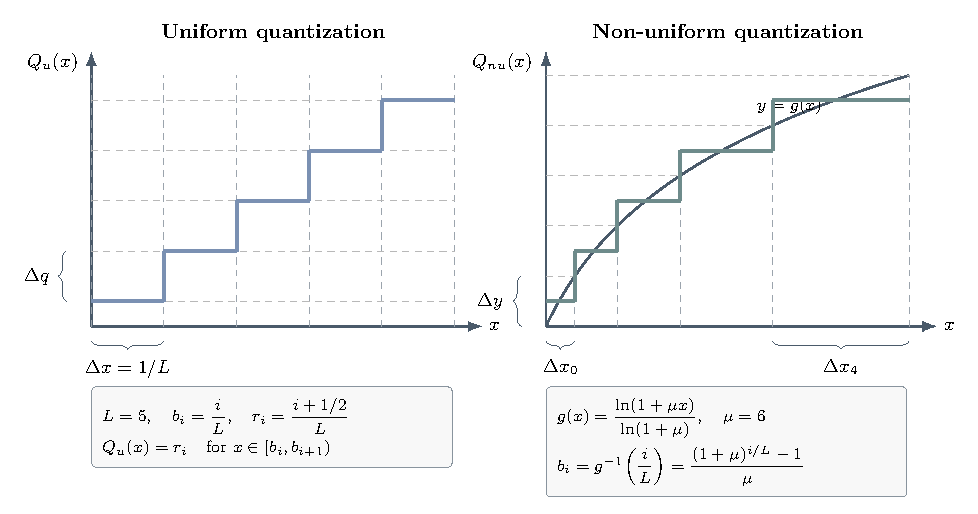
\includegraphics[width=\textwidth]{figures/compression/quantization.pdf}
  \caption{Uniform quantization (left) divides the input range into $L$ equal-width bins, assigning each interval $[b_i, b_{i+1})$ to a fixed representative $r_i$. Non-uniform quantization (right) applies a companding function $g(x)$ to warp the input space, allocating finer resolution at lower magnitudes where values concentrate and coarser bins at higher magnitudes.}
  \label{fig:quantization_example}
\end{figure}

\begin{table}[t]
\centering
\caption{Standard numerical formats commonly used in neural network quantization \cite{ieee754_2019,kalamkar2019bfloat16,jacob2018quantization,krishnamoorthi2018quantizing,lin2024awq}. The integer ranges correspond to signed stored integer values before dequantization; the represented real-valued range depends on the quantization scale and, when used, the zero-point.}
\label{tab:numerical_formats_quantization}
\begin{tabular}{lcccl}
  \toprule
  \textbf{Format} & \textbf{Bit-width} & \textbf{Type} & \textbf{Range} & \textbf{Typical application} \\
  \midrule
  FP32 & 32 & Floating point & $\sim \pm 10^{38}$ & Full-precision training baseline \\
  BF16 & 16 & Floating point & $\sim \pm 10^{38}$ & Mixed-precision training \\
  INT8 & 8  & Integer        & $[-128, 127]$      & Standard quantized inference \\
  INT4 & 4  & Integer        & $[-8, 7]$          & Aggressive low-bit compression \\
  \bottomrule
\end{tabular}
\end{table}

\FloatBarrier
\section{Neural Network Pruning}

Pruning is the process of reducing the size of a neural network by eliminating either connections or components that are responsible for outputting only a small proportion of the overall model prediction. The principle behind pruning relies on the observation that overparameterized neural networks (especially deep ones) generally do not require all the units and connections in order to achieve a good performance. Pruning can therefore reduce the storage space and computational cost to produce a less resource-intensive network.
\subsection{Formal Problem Formulation}

Given a parameterized network $f(\cdot;\Theta)$ whose $P$ parameters are
stored in $\Theta \in \mathbb{R}^P$, a binary mask $M \in \{0,1\}^P$ is
chosen such that those parameters selected to be kept (whose mask value is
$1$) can be retrieved and those not (mask value $0$) excluded from further
calculation by computing $f(x; M \odot \Theta)$, which zeros out parameters
for which $M_i = 0$ by elementwise product.

The goal is then to find the mask $M$ and the remaining weights $\Theta$ that
keep the loss $\mathcal{L}$ as low as possible while meeting a budget on how
many parameters are retained:
\begin{equation}
	\min_{\Theta, M}\; \mathcal{L}(M \odot \Theta)
	\quad
	\text{subject to}
	\quad
	\frac{\lVert M \rVert_0}{P} \le \kappa,
	\label{eq:constrained}
\end{equation}
where $\lVert M \rVert_0$ counts the nonzero entries of $M$ and $\kappa \in
(0,1]$ is the target density. In practice this hard constraint is often
replaced by a regularised objective that avoids having to fix $\kappa$ in
advance:
\begin{equation}
	\min_{\Theta, M}\; \mathcal{L}(M \odot \Theta) + \lambda\,\Omega(M),
	\label{eq:regularised}
\end{equation}
where $\lambda$ controls how aggressively compression is penalised and
$\Omega(M)$ can capture parameter count, memory footprint, or latency
depending on the deployment target. This regularised form folds the budget into the objective instead of enforcing it as a hard constraint (Eq.~\eqref{eq:regularised}).

Finding an optimal pruning solution is generally NP-hard, since the search
space grows exponentially with the number of parameters~\cite{dong2017learning}.
Practical methods thus resort to approximate measures which evaluate how pruning a parameter or structure affects performance without considering all possible masks. Such measures can be obtained by approximating the change in training loss due to pruning, commonly through a Taylor expansion \cite{molchanov2017variational}.

\subsection{Structural Forms of Pruning}
\label{sec:pruning_structures}

The binary mask in Eq.~\eqref{eq:constrained} indicates which elements in
the network need to be removed, but it does not indicate the pattern of
removal. The zeroes in $M$ may show up as discrete individual parameters, as
repetitive local structures, or as entire computational blocks. This leads to
the three typical types of pruning: unstructured, semi-structured and
structured pruning.

\begin{itemize}
    \item \textbf{Unstructured pruning} uses the mask at the level of
    individual weights. Each weight can be kept or removed independently, so
    the tensor dimensions remain unchanged while some entries are set to zero.

    \item \textbf{Semi-structured pruning} partitions a weight tensor into
    small blocks and applies the same rule to each block. In an $N\!:\!M$
    pattern, every block of $M$ weights keeps $N$ entries and removes the
    remaining $M-N$. For example, in a $2\!:\!4$ pattern, a group of four
    weights $(w_1,w_2,w_3,w_4)$ may receive a mask such as $(1,0,1,0)$,
    meaning that $w_1$ and $w_3$ are kept while $w_2$ and $w_4$ are removed.
    The same counting rule is then repeated across the tensor, block after
    block.

    \item \textbf{Structured pruning} applies the mask to complete
    computational units. These units may be neurons, groups of neurons,
    hidden dimensions, or full layers. Removing such units also removes the
    parameters attached to them, which naturally changes the dimensions of the
    affected parts of the network.
\end{itemize}

Thus, after the pruning objective has been written in terms of a mask, the
next distinction is the form taken by that mask inside the network: isolated
entries, repeated local groups, or complete units, as illustrated in
Figure~\ref{fig:structures}.

\begin{figure}[H]
    \centering
    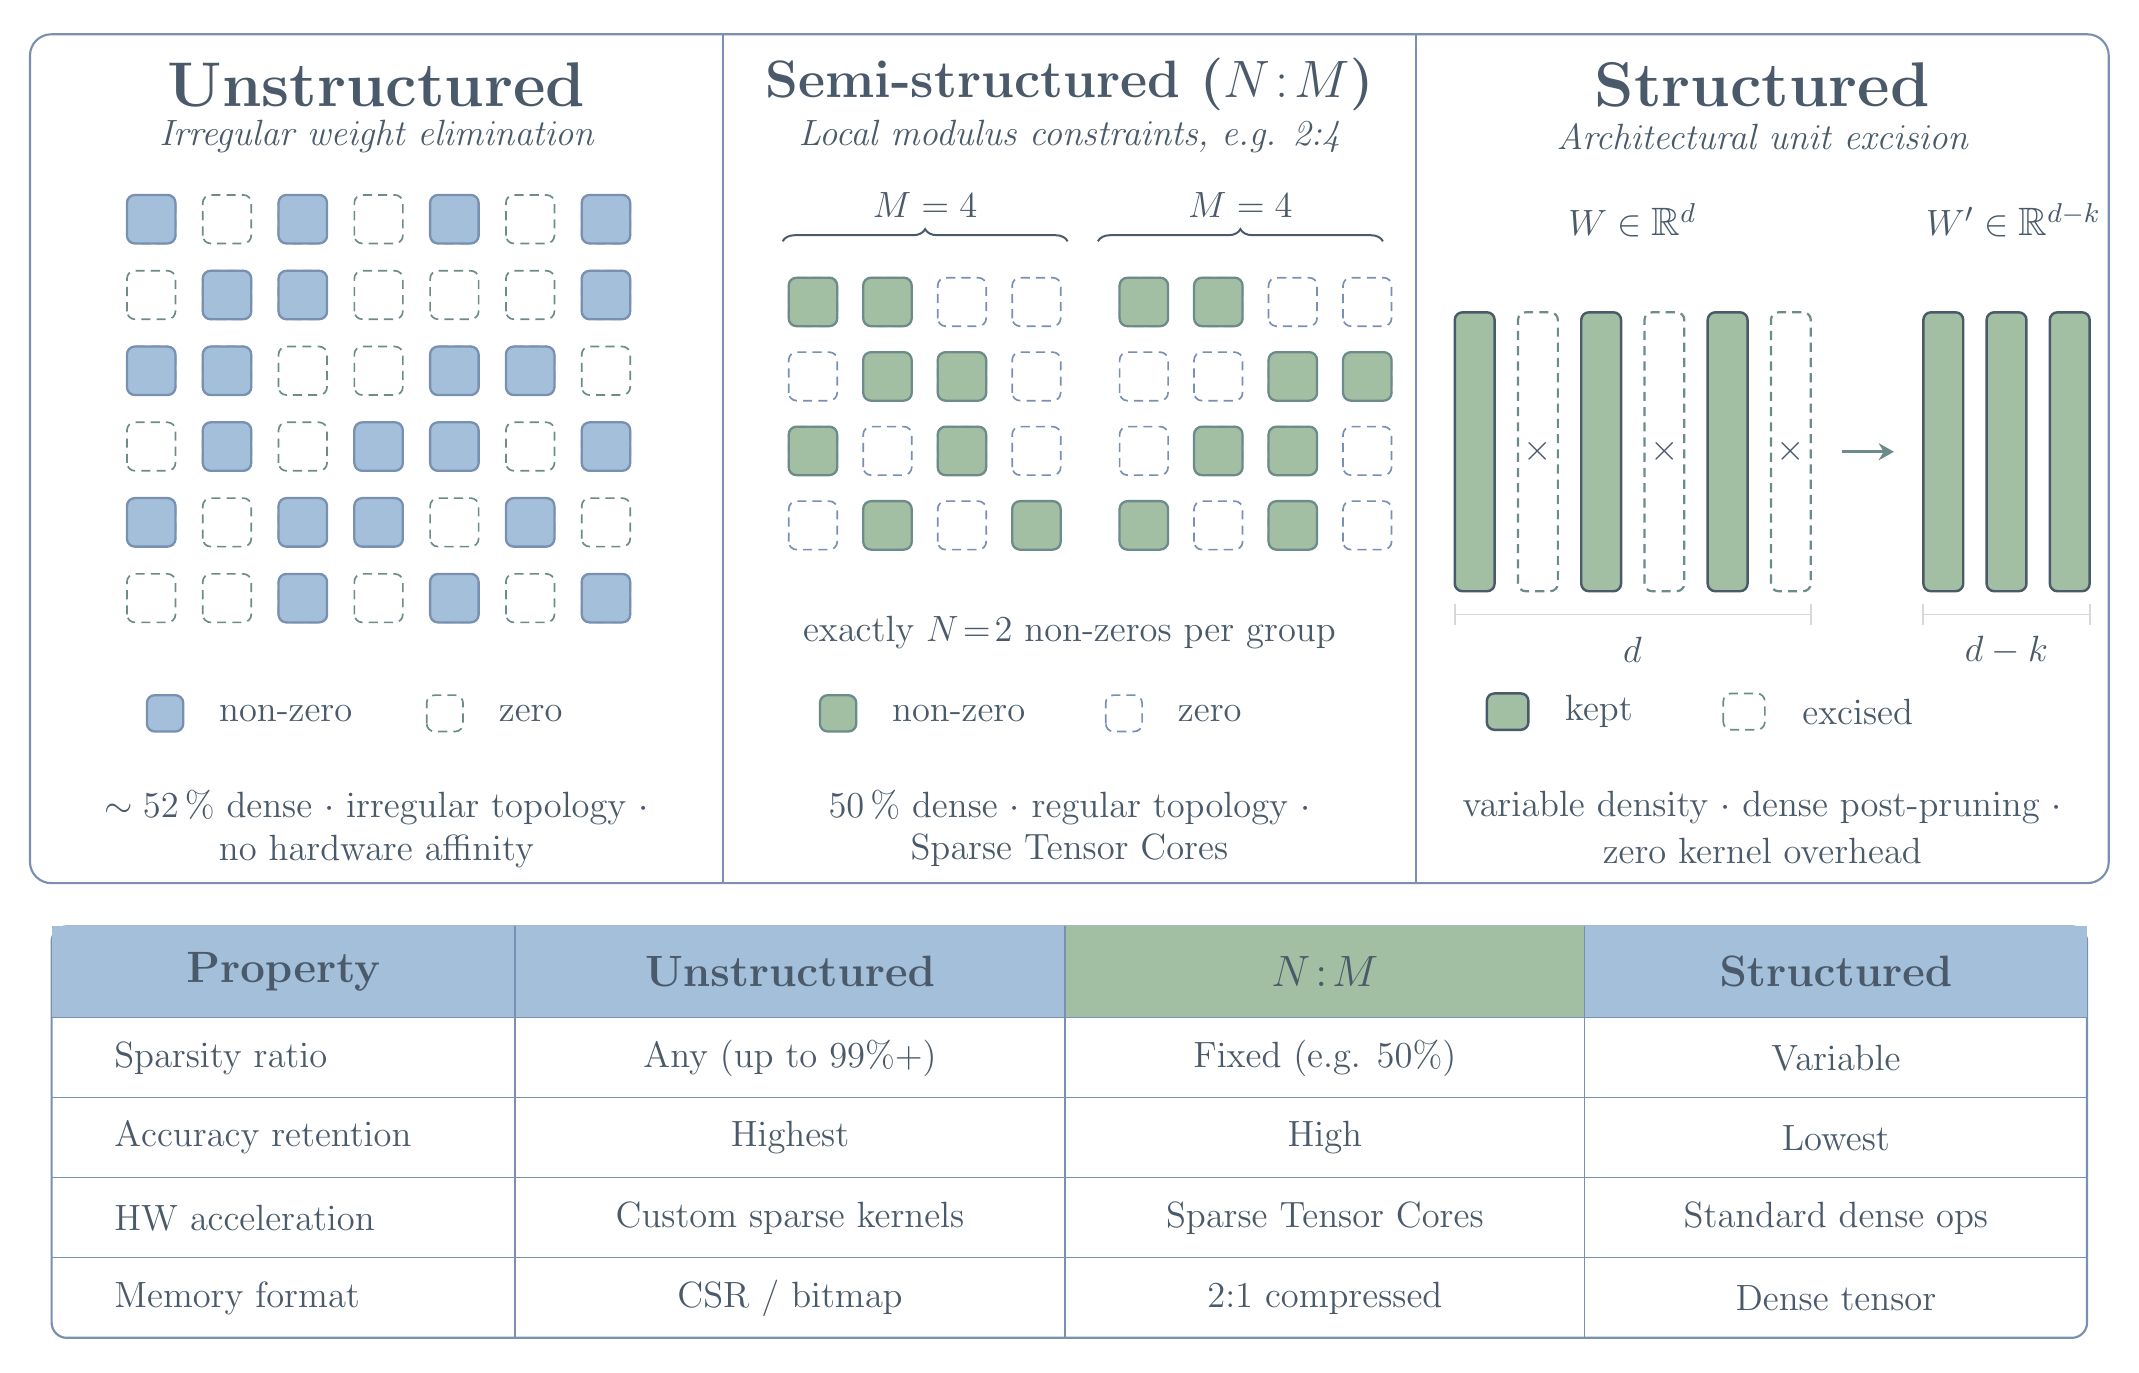
\includegraphics[width=0.75\textwidth]{figures/compression/pruning_s_ss_ns.PNG}
    \caption{A dense weight matrix can be pruned into unstructured sparsity,
        semi-structured 2:4 sparsity, or structured row, column, and block
        sparsity. The distinction is important at deployment time because
        increasingly regular sparsity patterns align more directly with
        accelerator execution primitives.}
    \label{fig:structures}
\end{figure}

\section{Low-Rank Factorization}

Low-rank factorization is a method for compressing high dimensional weight matrices by factorizing them into two or more lower dimensional matrices. This leverages the fact that a lot of weight matrices found in learned neural networks tend to be of a low rank, implying that the encoded information is residing on a lower dimensional manifold within the high dimensional parameter space \cite{li2018measuring}. By explicitly factorizing these matrices, the parameter space and the cost of matrix multiplications can be lowered.

\subsection{Mathematical Formulation}

Consider a weight matrix $W \in \mathbb{R}^{m \times n}$ of a pre-trained layer. We seek to approximate $W$ using two factor matrices $A \in \mathbb{R}^{m \times r}$ and $B \in \mathbb{R}^{r \times n}$, where $r$ is the rank and $r \ll \min(m, n)$. The approximation is given by:
\begin{equation}
  W \approx AB.
  \label{eq:lowrank_basic}
\end{equation}

The optimization objective is to minimize the reconstruction error, typically measured by the Frobenius norm:
\begin{equation}
  \min_{A,B} \|W - AB\|_F^2.
  \label{eq:factorization_opt}
\end{equation}

Ideally, the optimal solution is provided by the truncated Singular Value Decomposition (SVD). If $W = U \Sigma V^T$, the best rank-$r$ approximation is $U_r \Sigma_r V_r^T$, where $\Sigma_r$ contains the top $r$ singular values. In practice, $A$ and $B$ can be learned directly via gradient descent, or initialized via SVD and then fine-tuned.

The compression ratio achieved is defined as:
\begin{equation}
    C_{\text{ratio}} = \frac{mn}{r(m+n)},
\end{equation}
where $mn$ is the parameter count of the original matrix and $r(m+n)$ is the total count of the two factor matrices. For square matrices where $m=n$, the complexity reduces from $O(n^2)$ to $O(rn)$, offering linear scaling with respect to dimensionality when $r$ is constant.

\subsection{Applications}

As described in the formulation above, substituting a network's weight matrices with their low-rank approximations (Eq.~\ref{eq:lowrank_basic}) directly yields a compressed model~\cite{eckart1936approximation,xue2013restructuring,sainath2013lowrank}. The approach works best in layers where the weight matrix is already close to low-rank in practice, meaning a small number of components is enough to reconstruct it accurately~\cite{eckart1936approximation,xue2013restructuring}.

Moreover, one of the most prominent modern uses of low-rank factorization is Parameter-Efficient Fine-Tuning (PEFT). In methods such as Low-Rank Adaptation (LoRA) \cite{hu2021lora}, the pre-trained weights $W_0$ are frozen, and a trainable low-rank update $\Delta W$ is injected into the forward pass. For an input $x$, the layer output $h$ becomes:
\begin{equation}
    h = W_0 x + \Delta W x = W_0 x + AB x.
\end{equation}
Here, $A$ is typically initialized from a Gaussian distribution and $B$ is initialized to zero, ensuring the training starts with the original model behavior. Figure~\ref{fig:lowrank_concept} illustrates the decomposition geometrically. This allows for the adaptation of massive models by optimizing only a fraction of the parameters.

\definecolor{mistyblue}{RGB}{173, 216, 230}
\definecolor{sagegreen}{RGB}{135, 175, 135}
\definecolor{dustyteal}{RGB}{95, 158, 160}
\definecolor{decompcol}{RGB}{25, 25, 112}
\definecolor{lowrankcol}{RGB}{47, 79, 79}

\begin{figure}[htbp]
  \centering
  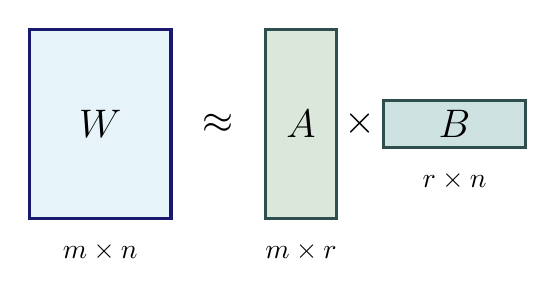
\begin{tikzpicture}[scale=0.6]
    % Original matrix
    \draw[fill=mistyblue!30, draw=decompcol, very thick] (0,0) rectangle (3,4);
    \node at (1.5,2) {\Large $W$};
    \node[below] at (1.5,-0.3) {$m \times n$};

    % Approximately equal
    \node at (4,2) {\Large $\approx$};

    % First factor
    \draw[fill=sagegreen!30, draw=lowrankcol, very thick] (5,0) rectangle (6.5,4);
    \node at (5.75,2) {\Large $A$};
    \node[below] at (5.75,-0.3) {$m \times r$};

    % Multiplication
    \node at (7,2) {\Large $\times$};

    % Second factor
    \draw[fill=dustyteal!30, draw=lowrankcol, very thick] (7.5,1.5) rectangle (10.5,2.5);
    \node at (9,2) {\Large $B$};
    \node[below] at (9,1.2) {$r \times n$};
  \end{tikzpicture}
  \caption{Schematic of Low-Rank Factorization. The dense matrix $W$ is decomposed into low-rank components $A$ and $B$, significantly reducing parameter count when $r \ll m, n$.}
  \label{fig:lowrank_concept}
\end{figure}

\section{Knowledge Distillation}

Knowledge Distillation (KD) is a model compression technique in which a lightweight student model is trained to imitate a larger, higher-performing teacher model. Rather than relying only on hard ground-truth labels, KD transfers knowledge through the teacher's soft probability distributions~\cite{hinton2015distilling}. These probabilities can encode useful structure in the data manifold, since similar incorrect-class probabilities may reflect semantic or visual relationships, providing the student with a richer supervisory signal.

\subsection{Mathematical Formulation}

The standard distillation framework modifies the softmax function by introducing a temperature hyperparameter $T$. For a given input, let $z_t$ and $z_s$ be the logits of the teacher and student, respectively. The ``softened'' probability for class $i$, $q_i$, is computed as:
\begin{equation}
    q_i(z; T) = \frac{\exp(z_i / T)}{\sum_j \exp(z_j / T)}.
    \label{eq:softmax_temp}
\end{equation}
A higher $T$ produces a smoother probability distribution, emphasizing the relationships between non-target classes.

The training objective for the student is a linear combination of the standard task loss (typically Cross-Entropy against ground truth hard labels, $y$) and the distillation loss (typically Kullback-Leibler divergence between the student's and teacher's soft distributions). The total loss $\mathcal{L}_{\text{total}}$ is defined as:
\begin{equation}
    \mathcal{L}_{\text{total}} = \alpha T^2 \mathcal{L}_{\text{KD}}(q(z_t; T), q(z_s; T)) + (1-\alpha) \mathcal{L}_{\text{CE}}(y, q(z_s; 1)),
    \label{eq:kd_loss}
\end{equation}
where $\alpha$ is a balancing coefficient and the $T^2$ term scales the gradients to account for the magnitude change caused by the temperature scaling.

\subsection{Methodological Taxonomies}

Distillation methodologies are categorized by the source of knowledge transferred, the training scheme employed, and the algorithmic mechanism used to align representations.

\subsubsection{Knowledge Sources}
The source determines what information is extracted from the teacher.
\begin{itemize}
    \item \textbf{Logit-Based Distillation:} The student mimics the teacher's final prediction distribution \cite{hinton2015distilling}. The loss $L_{\text{logit}}$ is the KL divergence between softened logits. While simple, it offers no insight into intermediate reasoning.
    \item \textbf{Feature-Based Distillation:} The student aligns its intermediate activations with the teacher's \cite{Romero2014}. The loss $L_{\text{feature}}$ minimizes the distance (e.g., L2) between transformed feature maps. This guides the student through the teacher's step-by-step reasoning.
    \item \textbf{Similarity-Based Distillation:} The student learns the \emph{relationships} between data samples. The loss $L_{\text{similarity}}$ matches the angles or distances between pairs of features in the teacher's space to those in the student's space, capturing structural topology rather than absolute values.
\end{itemize}

\subsubsection{Training Schemes}
The scheme defines the interaction between teacher and student during optimization.
\begin{itemize}
    \item \textbf{Offline Distillation:} A two-stage process where a high-capacity teacher is pre-trained and frozen. The student is trained subsequently to mimic the static teacher. This is effective for utilizing proprietary models but incurs high pre-training costs.
    \item \textbf{Online Distillation:} Teacher and student are trained simultaneously from scratch, learning collaboratively from each other and the ground truth. This eliminates pre-training but can be unstable as the teacher is not fully converged.
    \item \textbf{Self-Distillation:} The network acts as its own teacher. Knowledge is transferred from deeper layers to shallower layers, or from previous epochs to the current one, serving as a powerful regularization technique without external models.
\end{itemize}

\subsubsection{Advanced Algorithms}
Advanced mechanisms refine how the knowledge transfer is executed.
\begin{itemize}
    \item \textbf{Attention-Based Distillation:} This method transfers spatial attention maps instead of full feature maps \cite{Zagoruyko2016}. It teaches the student where to focus and emphasizes saliency rather than raw activation values.
    \item \textbf{Contrastive Distillation:} Inspired by self-supervised learning, this pulls the student's representation of an input closer to the teacher's while pushing it away from negative samples (via InfoNCE loss). This improves structural alignment in the feature space.
    \item \textbf{Adaptive Distillation:} These methods dynamically adjust distillation parameters (such as loss weights or sample importance) during training. By focusing on harder examples or altering the teacher's influence over time, they optimize the transfer efficiency.
\end{itemize}

KD's major problems consist of what knowledge needs to be transferred, which algorithm to choose, and designing student and teacher architectures \cite{mansourian2025comprehensivesurveyknowledgedistillation}. Figure~\ref{fig:knowledge_distillation} presents a typical diagram of the teacher-student KD framework.

\begin{figure}[H]
    \centering
    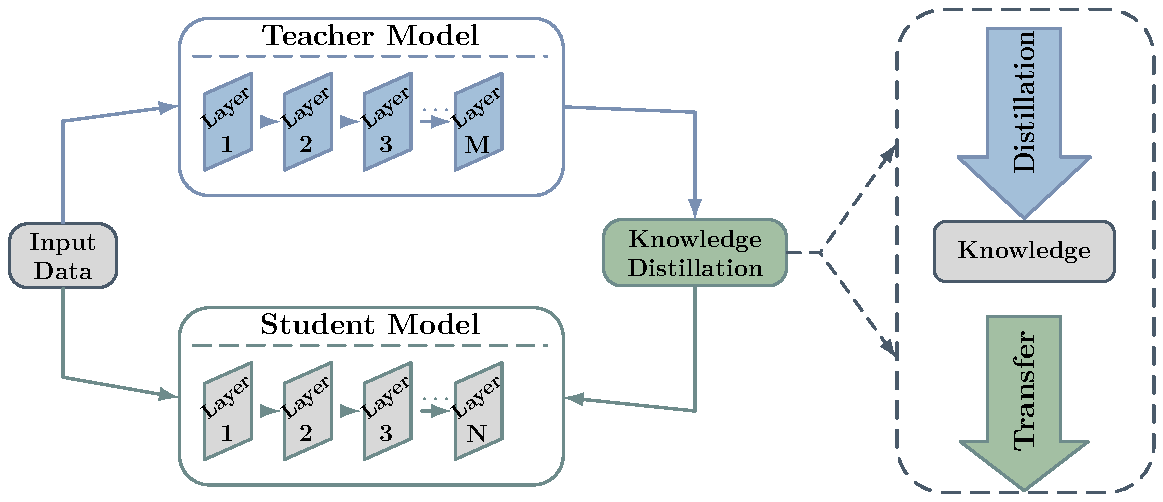
\includegraphics[width=\textwidth]{figures/compression/distill_diag.pdf}
    \caption{The Knowledge Distillation framework. The student minimizes a dual objective: the task loss $\mathcal{L}_{\text{task}}$ against hard labels and the distillation loss $\mathcal{L}_{KD}$ against the teacher's soft probability targets. Inspired from \cite{mansourian2025comprehensivesurveyknowledgedistillation}.}
    \label{fig:knowledge_distillation}
\end{figure}

\section{Conclusion}

This chapter discussed theoretical basis of model compression. We have presented the mathematical formulations and the structural taxons of Quantization, Pruning, Low-Rank Factorization and Distillation. All these compression techniques make use of redundancies in neural networks in order to achieve reduction in memory usage and computational costs. This evidence also shows that over-parameterized models can be reduced in size without losing predictiveness.

While the fundamental principles remain constant, practical deployment necessitates adaptation to specific architectures. In our case, the massive scale and unique attention mechanisms of the Transformer present distinct challenges. Consequently, the next chapter, \textit{Related Work}, investigates the empirical application of these concepts. It reviews the evolution of compression techniques specifically tailored for Large Language Models and Transformers and their optimization.
